\documentclass{book}
\usepackage[subpreambles=false]{standalone}

%%%%%%%%%%%%%%%%%%%%%%%%%%%
% Silence warning messages
\usepackage{silence}
\WarningsOff[scrlayer-notecolumn]
\WarningsOff[biblatex]

%%%%%%%%%%%%%%%%%%%%
% Commenting

%\usepackage[author=Lyndon]{pdfcomment}
%\newcommand{\pdfcomment}[1]{} %ignore all comments

%\usepackage{todonotes}
%\newcommand{\pdfcomment}{\todo}


%%%%%%%%%%%%%%%%%%%%
% Tables
\usepackage{booktabs}

%%%%%%%%%%%%%%%%%%%
% Fonts
\usepackage{tgadventor} %sans
\usepackage{tgpagella}  %serif
\usepackage{inconsolata} %mono
\usepackage[T1]{fontenc}

\usepackage{microtype}
\usepackage[all]{nowidow}
%%%%%%%%%%%%%%%%%%%%%%%
% Styling
\setcounter{secnumdepth}{4}
\setcounter{tocdepth}{2}

\usepackage{placeins}



%%%%%%%%%%%%%%%%%%%
% Math
\usepackage{amsmath, amssymb, stmaryrd, mathtools}
\DeclareMathOperator*{\argmin}{argmin}
\DeclareMathOperator*{\argmax}{argmax}

\usepackage{xparse,xstring,etoolbox}
% crossref this against notation section
\newcommand{\vv}[1]{\tilde{#1}} % vector
\newcommand{\seq}[1]{\mathcal{#1}} % sequence
\newcommand{\set}[1]{\mathbb{#1}} % set

%%%%%%%%%
% Indexing/sequence indexing
\newcommand{\seqind}[2]{#1^{#2}} % seqence index
\newcommand{\ind}[2]{#1_{#2}} % indexed
\newcommand{\disamb}[2]{#1^{\mathrm{#2}}} %disambiguated

%% Smart indexing and naming
\newcommand{\ifupper}[3]{
    \normalexpandarg
	\exploregroups
	\StrCount{ABCDEFGHIJKLMNOPQRSTUVWXYZ}{#1}[\uppercount]
	\ifnumgreater{\uppercount}{0}{#2}{#3}
}

%smart index
\DeclareDocumentCommand{\ii}{u{_} m}{
	\ifupper{#1}%
	{% just a single uppercase character, i.e. a matrix
		  %make sure the index is the right length
		\StrCount{#2}{,}[\indcount]
		\ifnumgreater{\indcount}{0}
		{ % Got multiple indexes so all good
		 	\ind{#1}{#2}
		}
		{ % Only 1 index so grab the column
		 	\ind{#1}{{:,#2}}
		}
	}%
	{% Not just a single upper case character
		\ind{#1}{#2}
	}
}

\DeclareDocumentCommand{\nn}{u{_} m}{
	\seqind{#1}{#2}
}

\DeclareDocumentCommand{\dd}{u{_} m}{
	\disamb{#1}{#2}
}

% Index of a vector
\DeclareDocumentCommand{\iv}{u{_} m}{\ii{\vv #1}_{#2}}
\DeclareDocumentCommand{\dv}{u{_} m}{\dd{\vv #1}_{#2}}
\DeclareDocumentCommand{\nv}{u{_} m}{\nn{\vv #1}_{#2}}

%exp
\let\oldexp\exp
\renewcommand{\exp}[1]{\oldexp \left( #1 \right)}
\newcommand{\exptwo}[1]{\oldexp_2 \left( #1 \right)}

\newcommand{\softmax}{\mathrm{smax}}

\DeclareMathOperator*{\expectedop}{\mathbb{E}}
\DeclareDocumentCommand{\expected}{u{_} m}{
	\expectedop\limits_{\mathrlap{#2}}
}

%%%%%%%%%%%%%%%%
%Graphics
\usepackage{tikz}
\usetikzlibrary{positioning, fit,  shapes.geometric}
\usepackage{ifthen}
\usepackage{etoolbox}

\tikzset{
	backgroundcolor/.style ={fill=white},
	every node/.append style={
		minimum height=7mm,
	},
	labe/.append style={
		%Blue,
		align = center,
		backgroundcolor,
		fill opacity=0.6,
		text opacity=1,
		font={\footnotesize\itshape}	
	},
	layer/.append style={
		draw,
		align = center,
		minimum height=7mm,
	},
	tight/.append style={
		inner sep=0.2mm,
	},
	lookupbox/.append style={
		draw=none,
		append after command={
		       	[shorten <= -0.5\pgflinewidth]
		       	([shift={(-1.5\pgflinewidth,-0.5\pgflinewidth)}]\tikzlastnode.north east)
		       	edge([shift={( 0.5\pgflinewidth,-0.5\pgflinewidth)}]\tikzlastnode.north west) 
		       	([shift={( 0.5\pgflinewidth,-0.5\pgflinewidth)}]\tikzlastnode.north west)
		       	edge([shift={( 0.5\pgflinewidth,-1.5\pgflinewidth)}]\tikzlastnode.south west)            
		       	([shift={( -1.5\pgflinewidth,+0.5\pgflinewidth)}]\tikzlastnode.south east)
		       	edge([shift={(-1.5\pgflinewidth,-0.5\pgflinewidth)}]\tikzlastnode.north east)
		},
		inner sep=0.7mm,
		outer sep=0mm,
		minimum width=25mm
	}
}

\usepackage{pgfplots}
\pgfplotsset{compat=1.14}
\pgfplotsset{sideplot/.append style={
		width=\notescolwidth,
		domain=-10:10,
		samples=101,
		smooth,
		enlarge y limits={abs=2},
		axis lines=middle,
		xlabel  = $z$,
		ylabel  = $y$,
	},
	equ/.append style={
		color=blue,
		thick,
		mark=none
	}
}

% Function  For a plot 
% it  needs to be declared in preamble because of how \makenote* interacts with multiple files
\def\errorsurface(#1,#2){(0.5*#1 + 0.7*#2 + sin(deg(1.5*#1 + #2^2)))^2}


\usepackage{graphicx}
\graphicspath{{./figs/}, {./}, {./figs/chaptersentencerrepr/}, {./figs/chapterintromachinelearning/}, {./figs/chapterwordrepr/}}
\usepackage{adjustbox}


%%%%%%%%%%%%%%%%%%%
% Refs
\usepackage{cleveref}

\addbibresource{master.bib}

%%%%%%%%%%%%%%%%%%%%
% Formatting

% for examples from natural language space.
\newcommand{\natlang}[1]{\ifmmode \text{``\texttt{#1}''} \else {``\texttt{#1}''}\fi}
% \ifmmode ``trick'' from https://tex.stackexchange.com/a/15194/5834

%%%%%%%%%%%%%%%%%%%%%



\begin{document}
\part{Conclusion}
\chapter{Conclusion}
Current research in natural language understanding relies on creating computer manipulatable representations of natural language for purposes of making inferences about meaning.


While, the normal machine learning adage that given enough data and a model with sufficiently high representational capacity any problem can be solved always applies,
we seem to have found a sweet spot, 
where a model seemingly without sufficiently high representational capacity,
never-the-less performs excellently on tasks with the amount of data that we have.
It seems clear that there will always exist various low-medium resource settings where this will be an ideal method for many problems.


The research presented here on linear combinations of embeddings has shown that this simple input representation technique is surprisingly powerful.
This surprising power come from the value of surface level information in many practical natural language understanding tasks.
The word content being the most obvious of these.
This word content is presented in a dense and informative form in a LCOWE; in a way that captures and preserves lexical similarity information.
While the LCOWE loses word order information, it very well preserves the word content.
That content proved more useful for the tasks considered in this research.


We considered a number of tasks to identify the utility of this representation in for different uses.
\Cref{SentVecMeaning} investigated classifying paraphrases as means to investigate quality of SOWE as a sentence embedding method.
\Cref{ColorEst} defined models for color estimation from short phrases.
\Cref{RefittingSenses} considered if we could use weighted combinations of sense embeddings to better capture the sense used in a particular example.
\Cref{NovelPerspective} considered taking the mean of the embeddings adjacent to named entity tokens across a fictional text as a feature to characterize how the named entity token was being used.
We followed up these practical demonstrations of capacity,
with further investigations into what can be recovered from the SOWE for the important category of sentence representations.
\Cref{BOWgen} demonstrated a method that could partially recover bags of words.
\Cref{SOWE2Sent} extended this to attempt to order those bags of words into sentences.
This demonstrated that a surprising amount of information is still available in the summed embeddings; which helps to explain why they work so well.



While it is clear that such linear combinations of embedding  representation spaces are not perfect for representing all meanings,
they are pragmatically very strong.
They do not encode any information about word order.
It is thus clear that there exist sentences and phrases that are ambiguous when represented this way.
However, we note that such sentences are rare: often there is only one likely ordering, particularly in any given  a restricted context.
Most sentences are relatively short; multiple similarly likely word ordering occur more often in longer sentences.
Many reorderings are paraphrases, or near paraphrases, particularly when done at the clause level.
Though some orderings, such as noun swaps of nouns with similar ontological classification (e.g. Agents, Objects) do exist at almost all lengths:
many are paraphrases \natlang{The banana is next to the orange.} vs \natlang{The orange is next to the banana};
and others are similar in meaning: \natlang{The banana is the left of the orange.} vs \natlang{The orange is the left of the banana}.
It is desirable that such sentences are near by in a representational of semantic space.

\section{Some reflections upon semantic spaces}
\begin{figure}
	\centering
	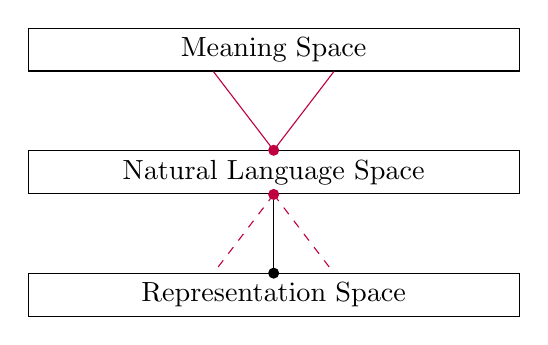
\begin{tikzpicture}[
	every node/.style = {text width=60mm,  align=center},
	pointdot/.style = {fill=purple, circle, minimum size=4pt,text width=0mm, inner sep=0pt}			
	]
	\node[draw](idea){Meaning Space};
	% Objects: ideas, thoughts
	\node[draw, below = of idea](nl){Natural Language Space};
	% Objects: utterances, sentences, words
	\node[draw, below = of nl](emb){Representation Space};
	% Objects: Embeddings
	
	\draw[purple] (idea.200) to (nl.north);
	\draw[purple] (idea.-20) to (nl.north);
	\node[pointdot] at (nl.north) {};
	
	\draw[] (nl) to (emb);
	\draw[dashed,purple] (nl.south) to (emb.20);
	\draw[dashed,purple] (nl.south) to (emb.-200);
	\node[pointdot] at (nl.south) {};
	
	\node[pointdot,black] at (emb.north) {};
	
	\end{tikzpicture}
	\caption{\label{fig:spaces} The representation space is a computationally manipulate representation of the meaning space.
		The natural language utterances come from points in the meaning space; though due to ambiguity we can only truly hope to estimate distributions when the interpret them. A single point embedding as an approximation to a distribution with a single tight peak.}
\end{figure}

We can consider that there is a true semantic space of ideas.
When speaking, this space is projected down to natural languages space.
To again quote Webber: ``A sentence is a group of words expressing a complete thought.'', it is not a complete thought, only the \emph{expression} of one.
This projection from idea to utterance is imperfect -- it is lossy.
Many ideas are expressed the same way, and language thus has a lot of ambiguity.
When we try to understand the meaning of a natural language utterance we are trying to find the point in meaning space that the speaker intend.
Some times the natural language space alone, is enough to recover a good idea of the the point in meaning space the speaker intends,
but other times it is not.

The preimage of a point in natural language space (e.g. a sentence),
is a probability distribution over meaning space that could have lead to that utterance -- $P(meaning \mid utterance)$.
This distribution could be combined with other factors (in a Bayesian way); either from that natural language context, or the enviroment more broadly.
For example, to use a meaning that centres around word sense:
we can identify two (of the many) senses of the word \natlang{apples}:
one in reference to the fruit, the other in reference to the computers made by the eponymous company.
Thus, on its own the sentence \natlang{Apples are good.}
suggests a distribution with at least two peaks in meaning space.
Combine that utterance, with the context of being in a computer store, rather than a grocer, and the probability of one peak can be increased, though  the other not entirely removed.
Further around each peak remains adjacent closely related possible meanings.
For example the statement could be in relation to only computers, or also to other products.
meaning space is a continuous space, with every utterance corresponding to a unique point. It is an uncountably large space.
In contrast natural language space is countably large, being composed of finite length combinations of of symbols taken from a finite alphabet.
An uncountable number of points in meaning space are projected down to a single point in natural language space.


When designing a embedding method, for sentences, words or other structures,
we seek to define a representation space
that has good 
In particular it should have a continuous mapping from to and from embedding space.
A neighbourhood in representation space, should correspond to a neighbourhood in meaning space.
\Cref{SentVecMeaning} investigated this for sentence embeddings.
By taking points in natural language space known to come from very near by points in meaning space, that is to say paraphrases,
and checking that they belong to near points in embedding space.


As each point in natural language space is defines a distribution over meaning space of what may be meant;
and representation space is attempting to be in correspondence to meaning space;
it is such that each point in natural language space should project to a distribution over embedding space.
Instead, most methods project to natural language points to single points in embeddings space.
This is viable when the region in meaning space that the natural language point could have come from is small -- in particular that the distribution in meaning space is narrow variance and mono-modal.
In that case the single point estimate in embedding space is an useful approximation.


This has particularly clear utility for word sense embeddings,
which are defined by multimodal distributions,
with large peaks for each homonym, and smaller nearby peaks for each polyseme.
Furthermore we can't rule out the speaker using the word incorrectly or metaphorically which gives rise to nonzero values elsewhere in meaning space.
Word-sense embeddings produce multiple sense embeddings -- ideally one corresponding to each peak in meaning space.
We know these peaks are only rough approximations to the true point in meaning space for a given usage of a word.
\Cref{RefittingSenses} attempts find other points in the embeddings space, that better corresponds to the true point in meaning space for the particular use.


Unsupervised methods, in particular word embeddings, but also more generally, are ungrounded.
They are based only on natural language space observations.
The goal is not to capture I meaning in this space,
but rather to create a space that is a good input to a supervised system that can learn a good correspondence from natural language space to meaning space. 
While we would not normally think of the SOWE sentence representation space as one for which there would be an easy alignment to the meaning space,
\Cref{SentVecMeaning} showed that it was.
A strong point in its favour is that it directly benefits from word embeddings.
Word embeddings are excellently suited for creating a space which, while ungrounded, has the internal consistency that makes it very useful as a representation space for supervision to be applied on top of.
It's great strength comes from Firth's distributional hypothesis, that words occurring in similar contexts have similar meaning.
While this does not allow the encoding of meaning itself, it does allow the encoding of similarity of meaning.
This is ideally suited for creating a space that will make a good source representation for a supervised method applied for natural language understanding task on words.
Were that task accomplished with a neural network, the later hidden layers, or the fine-turned embeddings would form a grounded representation of meaning space.
Our results show that that strength is carried forth into linear combinations of such embeddings.


The color understanding task considered in \Cref{ColorDist} is interesting.
While it is a typical natural language understanding system,
which takes a point in natural language space (a color name),
moves through a representation space (the output of one of the input modules: SOWE, CNN, or RNN) using supervision to output something from meaning space.
In this case the meaning space is very well grounded to the HSV color space.
We can, for many purposes, say for this natural language understanding task, the color space \emph{is} the meaning space.
Using point estimation it outputs a point in meaning space, reflecting (in some sense) the most reasonable guess of the meaning.
Using distribution estimation it outputs a distribution over the meaning space, fully reflecting the knowledge we have to infer the meaning.
The fact that even on the subset of the testing data where word order was ambiguous, SOWE was the best performing model highlights an important notion.
Word order ambiguity is just one amongst many sources of ambiguity in any representation of natural language.
In the color case, it boils down to the additional ambiguity of being unable to encode the word order difference between \natlang{bluish green} and \natlang{greenish blue}, is negligible compared to the inherent ambiguity in what either means.
Both phrases give rise to a large and overlapping distribution across meaning space.

In cases where there are multiple reasonable word orderings,
this means that multiple points in the true meaning space, correspond to a single point in the representational LCOWE space.
However, this is not exceptional: 
many sentences have two or more interpretations, a humours example being an accidental pun.
Thus even in a space that fully captures the natural language features, still a single point in that representational space
corresponds to two points in meaning space;
as the single point in natural language space could have come from either point in meaning space.
As such ambiguity from loss of word order is not an unique and unsalvageable problem.
If we thus had a distribution over meaning space, corresponding to the interpretation of a SOWE, it would have two peaks corresponding to two different word orders.
While such a discussion is purely theoretical as we do not have any way to generate such a distribution over true meaning space,
it remains interesting for in cases (like colors) where we have a well aligned near meaning space.
As we can use other contextual information define prior and thus decrease distributions associated with other ambiguities,
we can use language models to provide a prior over those peaks; based on the likelihood of word orders.
There exists a trivial extension of the work presented in \Cref{BOWgen,SOWE2Sent}, where the mixed integer programming model is constrained to give the second (and so forth) most likely solution, together with it's probability.
It is however not computationally practical, nor useful without a better meaning space representation.


While the research presented in this dissertation has made use of the idea that we are working with a sample from a distribution over a proxy for meaning space,
it is our belief that further advancements would benefit from fully considering
word embeddings and other objects from representation spaces, not as discrete points but as random variables with a linked distribution.
This however comes with significant challenges in that manipulating the very high dimensional distributions that are required for this is computationally challenging



\todo{Where does this paragraph belong?}
\Cref{SentVecMeaning} and \Cref{ColorEst} both consider represent contagious linguistic structures -- sentences and shore phrases respectively, as input representations.
Further, the output of the output modules discussed in \Cref{ColorEst} is a grounded representation space, though that work did not examine it directly.
\Cref{RefittingSenses} considers the representation of word senses, and it navigates this representation space to find new representations which better describe a particular use of a word.
\Cref{NovelPerspective} is more atypical:
the featuressets considered for the point of view detection task,
characterize how a particular named entity token was used throughout a chapter.
It is thus not a representation of the chapter meaning, as it varies for the different named entities.
It is in fact a representation of how that named entity is related to the events described in the chapter.
It seems like the MOWE feature set used in \Cref{NovelPerspective} it is vastly insufficient to represent such information given it is only a mean of the immediately adjacent words -- nothing like the whole chapter's contents.
However, as was demonstrated by the classical feature set considered in the same chapter, which primarily consisted of adjacent part of speech tag counts, and which also achieved very good results, surface information encodes a surprising amount of semantic depth.


\section{Future work}

\subsection{Adversarial Test cases}
It is worth consideration,
that adversarial test cases allow advancement of the state of the art to increase the capacity of models to represent all possibly inputs.
However, understanding how common they are are is essential.

Future work in this area requires not just the construction of adversarial examples; but of the determination of how common they are in practice.
Adversarial examples are not ubiquitous in real world tasks.
It is important not to succeed on only these cases, while failing on the more common simple cases.

It is also important to consider how adversarial such a challenging case is.
In \Cref{ColorEst}, the ordered task which was to make predictions for colors for which the different words in the name could appear in different orders to describe different colors.
For example \natlang{bluish green} and \natlang{greenish blue} are different colors.
However, they are very \emph{similar} colors.
As such the error from discarding word order, is less than the error from using a more complicated model such as an RNN.
Such a more complex model is harder to train, and those practical difficulties can dominate over a small amount of theoretical lack of capacity.



\section{Language Models and Orderless Representations}

There is a complementary aspect to LCOWE and language models.
While LCOWE have no capacity to handle word order but excellent ability to capture word content;
Pure language models have no ability to capture word content, but excellent ability to capture word order.
Language modelling based tasks incorporating a representation stage, such as encoder-decoders \citep{cho-EtAl:2014:EMNLP2014}, do not capture word content as well as LCOWE \citep{ac2018probingsentencevectors}.
They do, however, have state of the art order order representation.
\todo{I would really like to talk about how word embeddings are useful for caption evaluation here.}
%
%Future work in this area would be to enhance an encoder-decode model by concatenating to the shared state a SOWE.
%\todo{REDO this figure with the Embedding layers shown and the SOWE shared representation laye radded}
%
%
%
%\begin{figure}
%\begin{tikzpicture}
%	\numdef{\N}{8}
%	\numdef{\labelwidth}{5.5cm}
%
%	\node(lbl)[text width= \labelwidth] {\textbf{SOWE Enhanced\\RNN Encoder-Decoder}\\%
%		Variable $n$ inputs: $\nv x_t$\\%
%		Variable $m$ outputs $\nn \hat{y}_t$\\%
%		Prompts: $\nv r_t$ (often $y_{t-1}$)
%	};
%	
%	\coordinate[yshift = -3.5cm] (L0) at (lbl.west);
%	\numdef{\NN}{4}
%	\foreach \I[count=\j from 0] in {1,...,\NN}{
%		\ifnumequal{\I}{\NN - 1}{%
%			\node(L\I)[dashed, layer, right = of L\j] {\ldots};
%			\node(w\I)[below = of L\I]{\ldots};
%		}%
%		{
%			\node(L\I)[layer, right = of L\j] {$\mathrm{RU_E}$};
%			\node(w\I)[below = of L\I]{\ifnumequal{\I}{\NN}{$\nv x_n$}{$\nv x_\I$}};
%			\draw[->] (w\I) -- (L\I);
%		}
%	}
%	\foreach \I[count=\j from 1] in {2,...,\NN} {
%		\draw[->] (L\j) edge node[labe] {state} (L\I);
%	}
%	
%	
%	
%	
%	\coordinate[above = 3 of L\NN] (Lp\NN);
%	\numdef{\NP}{\N - 1}
%	\foreach \j in {\NN,...,\NP}{
%		\numdef{\I}{\j+1}
%		\numdef{\y}{\I - \NN}
%		\ifnumequal{\I}{\N-1}{%
%			\node(Lp\I)[dotted, layer, right = of Lp\j] {\ldots};
%			\node(w\I)[below = of Lp\I]{\ldots};
%			\node(y\I)[above = of Lp\I]{\ldots};
%			\draw[->,dotted] (w\I) -- (Lp\I);
%			\draw[->,dotted] (Lp\I) -- (y\I);
%			\path[->,dotted] (L\NN.north) edge node[labe]{$\vv z$} (w\I.south west);
%		}%
%		{
%			\node(Lp\I)[layer, right = of Lp\j] {$\mathrm{RU_D}$};
%			\ifnumequal{\I}{\N}{
%				\node(w\I)[below = of Lp\I]{$[\vv z; \nv r_m]$};
%				\node(y\I)[above = of Lp\I]{$\nn \hat{y}_m$};
%			}
%			{
%				\node(w\I)[below = of Lp\I]{$[\vv z; \nv r_\y]$};
%				\node(y\I)[above = of Lp\I]{$\nn \hat{y}_\y$};
%			}
%			
%			\draw[->] (w\I) -- (Lp\I);
%			\draw[->] (Lp\I) -- (y\I);
%			\path[->] (L\NN.north) edge node[labe]{$\vv z$} (w\I.south west);
%		}
%	}
%	
%	
%	\numdef{\NNp1}{\NN + 1}
%	\foreach \I in {\NNp1,...,\NP} {
%		\numdef{\j}{\I+1}
%		\draw[->] (Lp\I) edge node[labe] {state} (Lp\j);
%	}
%\end{tikzpicture}
%
%\end{figure}




\end{document}